\documentclass[twoside]{book}

% Packages required by doxygen
\usepackage{fixltx2e}
\usepackage{calc}
\usepackage{doxygen}
\usepackage[export]{adjustbox} % also loads graphicx
\usepackage{graphicx}
\usepackage[utf8]{inputenc}
\usepackage{makeidx}
\usepackage{multicol}
\usepackage{multirow}
\PassOptionsToPackage{warn}{textcomp}
\usepackage{textcomp}
\usepackage[nointegrals]{wasysym}
\usepackage[table]{xcolor}

% Font selection
\usepackage[T1]{fontenc}
\usepackage[scaled=.90]{helvet}
\usepackage{courier}
\usepackage{amssymb}
\usepackage{sectsty}
\renewcommand{\familydefault}{\sfdefault}
\allsectionsfont{%
  \fontseries{bc}\selectfont%
  \color{darkgray}%
}
\renewcommand{\DoxyLabelFont}{%
  \fontseries{bc}\selectfont%
  \color{darkgray}%
}
\newcommand{\+}{\discretionary{\mbox{\scriptsize$\hookleftarrow$}}{}{}}

% Page & text layout
\usepackage{geometry}
\geometry{%
  a4paper,%
  top=2.5cm,%
  bottom=2.5cm,%
  left=2.5cm,%
  right=2.5cm%
}
\tolerance=750
\hfuzz=15pt
\hbadness=750
\setlength{\emergencystretch}{15pt}
\setlength{\parindent}{0cm}
\setlength{\parskip}{3ex plus 2ex minus 2ex}
\makeatletter
\renewcommand{\paragraph}{%
  \@startsection{paragraph}{4}{0ex}{-1.0ex}{1.0ex}{%
    \normalfont\normalsize\bfseries\SS@parafont%
  }%
}
\renewcommand{\subparagraph}{%
  \@startsection{subparagraph}{5}{0ex}{-1.0ex}{1.0ex}{%
    \normalfont\normalsize\bfseries\SS@subparafont%
  }%
}
\makeatother

% Headers & footers
\usepackage{fancyhdr}
\pagestyle{fancyplain}
\fancyhead[LE]{\fancyplain{}{\bfseries\thepage}}
\fancyhead[CE]{\fancyplain{}{}}
\fancyhead[RE]{\fancyplain{}{\bfseries\leftmark}}
\fancyhead[LO]{\fancyplain{}{\bfseries\rightmark}}
\fancyhead[CO]{\fancyplain{}{}}
\fancyhead[RO]{\fancyplain{}{\bfseries\thepage}}
\fancyfoot[LE]{\fancyplain{}{}}
\fancyfoot[CE]{\fancyplain{}{}}
\fancyfoot[RE]{\fancyplain{}{\bfseries\scriptsize Generated by Doxygen }}
\fancyfoot[LO]{\fancyplain{}{\bfseries\scriptsize Generated by Doxygen }}
\fancyfoot[CO]{\fancyplain{}{}}
\fancyfoot[RO]{\fancyplain{}{}}
\renewcommand{\footrulewidth}{0.4pt}
\renewcommand{\chaptermark}[1]{%
  \markboth{#1}{}%
}
\renewcommand{\sectionmark}[1]{%
  \markright{\thesection\ #1}%
}

% Indices & bibliography
\usepackage{natbib}
\usepackage[titles]{tocloft}
\setcounter{tocdepth}{3}
\setcounter{secnumdepth}{5}
\makeindex

% Hyperlinks (required, but should be loaded last)
\usepackage{ifpdf}
\ifpdf
  \usepackage[pdftex,pagebackref=true]{hyperref}
\else
  \usepackage[ps2pdf,pagebackref=true]{hyperref}
\fi
\hypersetup{%
  colorlinks=true,%
  linkcolor=blue,%
  citecolor=blue,%
  unicode%
}

% Custom commands
\newcommand{\clearemptydoublepage}{%
  \newpage{\pagestyle{empty}\cleardoublepage}%
}

\usepackage{caption}
\captionsetup{labelsep=space,justification=centering,font={bf},singlelinecheck=off,skip=4pt,position=top}

%===== C O N T E N T S =====

\begin{document}

% Titlepage & ToC
\hypersetup{pageanchor=false,
             bookmarksnumbered=true,
             pdfencoding=unicode
            }
\pagenumbering{roman}
\begin{titlepage}
\vspace*{7cm}
\begin{center}%
{\Large Kjapp gamelobby }\\
\vspace*{1cm}
{\large Generated by Doxygen 1.8.11}\\
\end{center}
\end{titlepage}
\clearemptydoublepage
\tableofcontents
\clearemptydoublepage
\pagenumbering{arabic}
\hypersetup{pageanchor=true}

%--- Begin generated contents ---
\chapter{Namespace Index}
\section{Namespace List}
Here is a list of all documented namespaces with brief descriptions\+:\begin{DoxyCompactList}
\item\contentsline{section}{\hyperlink{namespacekjapp}{kjapp} \\*Contains all the resources needed to get kjapp game lobby system to work }{\pageref{namespacekjapp}}{}
\end{DoxyCompactList}

\chapter{Hierarchical Index}
\section{Class Hierarchy}
This inheritance list is sorted roughly, but not completely, alphabetically\+:\begin{DoxyCompactList}
\item \contentsline{section}{Curl\+Deleter}{\pageref{structCurlDeleter}}{}
\item \contentsline{section}{Scene}{\pageref{classScene}}{}
\begin{DoxyCompactList}
\item \contentsline{section}{Chat\+Client}{\pageref{classChatClient}}{}
\item \contentsline{section}{Chat\+Menu}{\pageref{classChatMenu}}{}
\item \contentsline{section}{Chat\+Room\+Lister}{\pageref{classChatRoomLister}}{}
\item \contentsline{section}{Chat\+Server}{\pageref{classChatServer}}{}
\item \contentsline{section}{Chat\+Server\+Configurator}{\pageref{classChatServerConfigurator}}{}
\end{DoxyCompactList}
\end{DoxyCompactList}

\chapter{Class Index}
\section{Class List}
Here are the classes, structs, unions and interfaces with brief descriptions\+:\begin{DoxyCompactList}
\item\contentsline{section}{\hyperlink{classChatClient}{Chat\+Client} }{\pageref{classChatClient}}{}
\item\contentsline{section}{\hyperlink{classChatMenu}{Chat\+Menu} }{\pageref{classChatMenu}}{}
\item\contentsline{section}{\hyperlink{classChatRoomLister}{Chat\+Room\+Lister} }{\pageref{classChatRoomLister}}{}
\item\contentsline{section}{\hyperlink{classChatServer}{Chat\+Server} }{\pageref{classChatServer}}{}
\item\contentsline{section}{\hyperlink{classChatServerConfigurator}{Chat\+Server\+Configurator} }{\pageref{classChatServerConfigurator}}{}
\item\contentsline{section}{\hyperlink{structCurlDeleter}{Curl\+Deleter} }{\pageref{structCurlDeleter}}{}
\item\contentsline{section}{\hyperlink{classScene}{Scene} }{\pageref{classScene}}{}
\end{DoxyCompactList}

\chapter{Namespace Documentation}
\hypertarget{namespacekjapp}{}\section{kjapp Namespace Reference}
\label{namespacekjapp}\index{kjapp@{kjapp}}


Contains all the resources needed to get kjapp game lobby system to work.  


\subsection*{Enumerations}
\begin{DoxyCompactItemize}
\item 
enum \hyperlink{namespacekjapp_a98b9b721617fe3ae75dd6f92507d2121}{Query} \{ \\*
\hyperlink{namespacekjapp_a98b9b721617fe3ae75dd6f92507d2121a446d73d3d33c027a52dea354cbb89f6a}{Query\+::\+A\+L\+L\+\_\+\+M\+A\+T\+C\+H\+ES}, 
\hyperlink{namespacekjapp_a98b9b721617fe3ae75dd6f92507d2121a18a470572636e1681c90bcfd186c90d1}{Query\+::\+N\+O\+T\+\_\+\+I\+N\+\_\+\+S\+E\+S\+S\+I\+ON}, 
\hyperlink{namespacekjapp_a98b9b721617fe3ae75dd6f92507d2121adb763e1606844ad7b28517112f999292}{Query\+::\+I\+N\+\_\+\+S\+E\+S\+S\+I\+ON}, 
\hyperlink{namespacekjapp_a98b9b721617fe3ae75dd6f92507d2121ae7b891a89f0e4fcea5a49f69d681ecf8}{Query\+::\+N\+O\+N\+\_\+\+F\+U\+L\+L\+\_\+\+M\+A\+T\+C\+H\+ES}, 
\\*
\hyperlink{namespacekjapp_a98b9b721617fe3ae75dd6f92507d2121a91d2f758dc36530a732923fcb757f4ab}{Query\+::\+B\+Y\+\_\+\+N\+A\+ME}
 \}\begin{DoxyCompactList}\small\item\em Different categories of queries that can be done on the kjapp database over matches. \end{DoxyCompactList}
\item 
enum \hyperlink{namespacekjapp_a424e0b2658aa21768d94092bc8155d5e}{Status} \{ {\bfseries N\+O\+T\+\_\+\+I\+N\+\_\+\+S\+E\+S\+S\+I\+ON}, 
{\bfseries I\+N\+\_\+\+S\+E\+S\+S\+I\+ON}
 \}\hypertarget{namespacekjapp_a424e0b2658aa21768d94092bc8155d5e}{}\label{namespacekjapp_a424e0b2658aa21768d94092bc8155d5e}
\begin{DoxyCompactList}\small\item\em The status of a match. Is it in session or not. \end{DoxyCompactList}
\end{DoxyCompactItemize}
\subsection*{Functions}
\begin{DoxyCompactItemize}
\item 
std\+::string \hyperlink{namespacekjapp_a60bf27524c6562d2eca46d8d2498aab4}{get\+My\+IP} ()
\begin{DoxyCompactList}\small\item\em Returns the external IP address of this computer. \end{DoxyCompactList}\item 
nlohmann\+::json \hyperlink{namespacekjapp_a22cf098842afd3b77a7c8635c26a7f95}{host\+Match} (const std\+::string \&game\+Token, const std\+::string \&name, const std\+::string \&host\+IP, const std\+::uint16\+\_\+t host\+Port, const std\+::size\+\_\+t max\+Player\+Count, const std\+::size\+\_\+t player\+Count=0, const std\+::string \&misc\+Info=\char`\"{} \char`\"{})
\begin{DoxyCompactList}\small\item\em Reports to the kjapp game lobby that a match has been created. \end{DoxyCompactList}\item 
std\+::vector$<$ nlohmann\+::json $>$ \hyperlink{namespacekjapp_a8eb2ba8b8328013a3e48b4427f602c8e}{get\+Matches} (const std\+::string \&game\+Token, \hyperlink{namespacekjapp_a98b9b721617fe3ae75dd6f92507d2121}{Query} query=\hyperlink{namespacekjapp_a98b9b721617fe3ae75dd6f92507d2121a446d73d3d33c027a52dea354cbb89f6a}{Query\+::\+A\+L\+L\+\_\+\+M\+A\+T\+C\+H\+ES}, const std\+::string \&name=\char`\"{}\char`\"{})
\begin{DoxyCompactList}\small\item\em Returns all the matches belonging to the specified game token that also fits within the specified query. \end{DoxyCompactList}\item 
void \hyperlink{namespacekjapp_afb16af4f3688ee259d2dad309ce65e9c}{delete\+Match} (const std\+::string \&game\+Token, const std\+::string \&match\+Id)
\begin{DoxyCompactList}\small\item\em Deletes the match with the id match\+Id, belonging to the game specified by game\+Token from the kjapp match database. \end{DoxyCompactList}\item 
void \hyperlink{namespacekjapp_aab9e24c5c8377e6ea59e261573a8886c}{update\+Match\+Status} (const std\+::string \&game\+Token, const std\+::string \&match\+Id, \hyperlink{namespacekjapp_a424e0b2658aa21768d94092bc8155d5e}{Status} status)
\begin{DoxyCompactList}\small\item\em Updates the status of the match belonging to the game with the specified game token, and identified by the specified match\+Id. \end{DoxyCompactList}\item 
void \hyperlink{namespacekjapp_ae7b42c3ae999b0f34c20202585ce7791}{update\+Player\+Count} (const std\+::string \&game\+Token, const std\+::string \&match\+Id, std\+::size\+\_\+t player\+Count)
\begin{DoxyCompactList}\small\item\em Updates the number of players of the match belonging to the game with the specified game token, and identified by the specified match\+Id. \end{DoxyCompactList}\item 
nlohmann\+::json \hyperlink{namespacekjapp_a1967229dd0630020ab4e19cab9b09d74}{post\+Match\+Report} (const std\+::string \&game\+Token, const std\+::string \&match\+Id, const nlohmann\+::json \&data)
\begin{DoxyCompactList}\small\item\em Sends a match report to the kjapp game lobby. \end{DoxyCompactList}\end{DoxyCompactItemize}


\subsection{Detailed Description}
Contains all the resources needed to get kjapp game lobby system to work. 

The kjapp game lobby system is a game lobby system that uses H\+T\+TP requests to communicate with a database. This namespace contains wrappers for these H\+T\+TP requests to allow developers to easily integrate simple lobby functionality into their games.

\begin{DoxyParagraph}{J\+S\+ON}
Kjapp in general uses a lot of json objects, as these are the ones that are most natural to work with when discussing H\+T\+TP web requests. For this we have decided on using nlohmann json library.
\end{DoxyParagraph}
\begin{DoxyParagraph}{libcurl}
For the H\+T\+TP requests we use libcurl.
\end{DoxyParagraph}
\begin{DoxyParagraph}{game tokens}
To use the kjapp game lobby system developers need to register their games, and apply for a game token. These tokens are api keys that are used by all kjapp functions to identify which game different matches and reports belong to. One can apply for a game token, but the token must be valid before it can be used for anything productive.
\end{DoxyParagraph}
\begin{DoxyParagraph}{Multiple threads}
The kjapp functions are blocking calls, and can be run in a separate thread. However, be careful about doing kjapp calls from multiple threads at the same time. Nothing in kjapp explicitly should cause any issues, but there might be situations where curl does not like it.
\end{DoxyParagraph}
\begin{DoxyParagraph}{Validation and Error handling}
Most validation happens on the server side of kjapp glm. However, to make it a bit easier to work with, the most common and easy to make errors results in an exception. These are mentioned in more detail in documentation of different functions. In general the rule is that if something is really obvious like game\+Token and match\+Id not having a length of 0 is not checked, but more hard to spot errors, like misc\+Info having a length of 0, will result in invalid argument exceptions. Any H\+T\+TP errors, like 404, will throw a runtime exception.
\end{DoxyParagraph}
\begin{DoxySeeAlso}{See also}
\href{https://github.com/nlohmann/json}{\tt nlohmann json} 

\href{https://curl.haxx.se/libcurl/c/libcurl.html}{\tt libcurl} 

\href{https://curl.haxx.se/libcurl/c/threadsafe.html}{\tt curl thread safety} 
\end{DoxySeeAlso}


\subsection{Enumeration Type Documentation}
\index{kjapp@{kjapp}!Query@{Query}}
\index{Query@{Query}!kjapp@{kjapp}}
\subsubsection[{\texorpdfstring{Query}{Query}}]{\setlength{\rightskip}{0pt plus 5cm}enum {\bf kjapp\+::\+Query}\hspace{0.3cm}{\ttfamily [strong]}}\hypertarget{namespacekjapp_a98b9b721617fe3ae75dd6f92507d2121}{}\label{namespacekjapp_a98b9b721617fe3ae75dd6f92507d2121}


Different categories of queries that can be done on the kjapp database over matches. 

\begin{Desc}
\item[Enumerator]\par
\begin{description}
\index{A\+L\+L\+\_\+\+M\+A\+T\+C\+H\+ES@{A\+L\+L\+\_\+\+M\+A\+T\+C\+H\+ES}!kjapp@{kjapp}}\index{kjapp@{kjapp}!A\+L\+L\+\_\+\+M\+A\+T\+C\+H\+ES@{A\+L\+L\+\_\+\+M\+A\+T\+C\+H\+ES}}\item[{\em 
A\+L\+L\+\_\+\+M\+A\+T\+C\+H\+ES\hypertarget{namespacekjapp_a98b9b721617fe3ae75dd6f92507d2121a446d73d3d33c027a52dea354cbb89f6a}{}\label{namespacekjapp_a98b9b721617fe3ae75dd6f92507d2121a446d73d3d33c027a52dea354cbb89f6a}
}]Gets all the matches belonging to a specified game token. \index{N\+O\+T\+\_\+\+I\+N\+\_\+\+S\+E\+S\+S\+I\+ON@{N\+O\+T\+\_\+\+I\+N\+\_\+\+S\+E\+S\+S\+I\+ON}!kjapp@{kjapp}}\index{kjapp@{kjapp}!N\+O\+T\+\_\+\+I\+N\+\_\+\+S\+E\+S\+S\+I\+ON@{N\+O\+T\+\_\+\+I\+N\+\_\+\+S\+E\+S\+S\+I\+ON}}\item[{\em 
N\+O\+T\+\_\+\+I\+N\+\_\+\+S\+E\+S\+S\+I\+ON\hypertarget{namespacekjapp_a98b9b721617fe3ae75dd6f92507d2121a18a470572636e1681c90bcfd186c90d1}{}\label{namespacekjapp_a98b9b721617fe3ae75dd6f92507d2121a18a470572636e1681c90bcfd186c90d1}
}]Gets all the matches belonging to a specified game token that are not in session.

This means that the match has not yet been started, or that it has been stopped. \index{I\+N\+\_\+\+S\+E\+S\+S\+I\+ON@{I\+N\+\_\+\+S\+E\+S\+S\+I\+ON}!kjapp@{kjapp}}\index{kjapp@{kjapp}!I\+N\+\_\+\+S\+E\+S\+S\+I\+ON@{I\+N\+\_\+\+S\+E\+S\+S\+I\+ON}}\item[{\em 
I\+N\+\_\+\+S\+E\+S\+S\+I\+ON\hypertarget{namespacekjapp_a98b9b721617fe3ae75dd6f92507d2121adb763e1606844ad7b28517112f999292}{}\label{namespacekjapp_a98b9b721617fe3ae75dd6f92507d2121adb763e1606844ad7b28517112f999292}
}]Gets all the matches belonging to a specified game token that are in session.

This means that the match is currently running. \index{N\+O\+N\+\_\+\+F\+U\+L\+L\+\_\+\+M\+A\+T\+C\+H\+ES@{N\+O\+N\+\_\+\+F\+U\+L\+L\+\_\+\+M\+A\+T\+C\+H\+ES}!kjapp@{kjapp}}\index{kjapp@{kjapp}!N\+O\+N\+\_\+\+F\+U\+L\+L\+\_\+\+M\+A\+T\+C\+H\+ES@{N\+O\+N\+\_\+\+F\+U\+L\+L\+\_\+\+M\+A\+T\+C\+H\+ES}}\item[{\em 
N\+O\+N\+\_\+\+F\+U\+L\+L\+\_\+\+M\+A\+T\+C\+H\+ES\hypertarget{namespacekjapp_a98b9b721617fe3ae75dd6f92507d2121ae7b891a89f0e4fcea5a49f69d681ecf8}{}\label{namespacekjapp_a98b9b721617fe3ae75dd6f92507d2121ae7b891a89f0e4fcea5a49f69d681ecf8}
}]Gets all the matches belonging to a specified game token that are not full. \index{B\+Y\+\_\+\+N\+A\+ME@{B\+Y\+\_\+\+N\+A\+ME}!kjapp@{kjapp}}\index{kjapp@{kjapp}!B\+Y\+\_\+\+N\+A\+ME@{B\+Y\+\_\+\+N\+A\+ME}}\item[{\em 
B\+Y\+\_\+\+N\+A\+ME\hypertarget{namespacekjapp_a98b9b721617fe3ae75dd6f92507d2121a91d2f758dc36530a732923fcb757f4ab}{}\label{namespacekjapp_a98b9b721617fe3ae75dd6f92507d2121a91d2f758dc36530a732923fcb757f4ab}
}]Gets all the matches belonging to a specified game token with a specified name. Both partial and full names can be specified. \end{description}
\end{Desc}


\subsection{Function Documentation}
\index{kjapp@{kjapp}!delete\+Match@{delete\+Match}}
\index{delete\+Match@{delete\+Match}!kjapp@{kjapp}}
\subsubsection[{\texorpdfstring{delete\+Match(const std\+::string \&game\+Token, const std\+::string \&match\+Id)}{deleteMatch(const std::string &gameToken, const std::string &matchId)}}]{\setlength{\rightskip}{0pt plus 5cm}void kjapp\+::delete\+Match (
\begin{DoxyParamCaption}
\item[{const std\+::string \&}]{game\+Token, }
\item[{const std\+::string \&}]{match\+Id}
\end{DoxyParamCaption}
)}\hypertarget{namespacekjapp_afb16af4f3688ee259d2dad309ce65e9c}{}\label{namespacekjapp_afb16af4f3688ee259d2dad309ce65e9c}


Deletes the match with the id match\+Id, belonging to the game specified by game\+Token from the kjapp match database. 

Informs the kjapp game lobby that a match should be deleted. The match is identified by the match\+Id and the game token.


\begin{DoxyParams}{Parameters}
{\em game\+Token} & The game\+Token of the game that the match to be deleted belongs to.\\
\hline
{\em match\+Id} & The id of the match that is supposed to be deleted.\\
\hline
\end{DoxyParams}

\begin{DoxyExceptions}{Exceptions}
{\em std\+::runtime\+\_\+exception} & 
\begin{DoxyItemize}
\item A curl handle couldn\textquotesingle{}t be created.
\item The H\+T\+TP request returned an error code, i.\+e. 40X 
\end{DoxyItemize}\\
\hline
\end{DoxyExceptions}
\index{kjapp@{kjapp}!get\+Matches@{get\+Matches}}
\index{get\+Matches@{get\+Matches}!kjapp@{kjapp}}
\subsubsection[{\texorpdfstring{get\+Matches(const std\+::string \&game\+Token, Query query=\+Query\+::\+A\+L\+L\+\_\+\+M\+A\+T\+C\+H\+E\+S, const std\+::string \&name="""")}{getMatches(const std::string &gameToken, Query query=Query::ALL_MATCHES, const std::string &name="")}}]{\setlength{\rightskip}{0pt plus 5cm}std\+::vector$<$ nlohmann\+::json $>$ kjapp\+::get\+Matches (
\begin{DoxyParamCaption}
\item[{const std\+::string \&}]{game\+Token, }
\item[{{\bf kjapp\+::\+Query}}]{query = {\ttfamily {\bf Query\+::\+A\+L\+L\+\_\+\+M\+A\+T\+C\+H\+ES}}, }
\item[{const std\+::string \&}]{name = {\ttfamily \char`\"{}\char`\"{}}}
\end{DoxyParamCaption}
)}\hypertarget{namespacekjapp_a8eb2ba8b8328013a3e48b4427f602c8e}{}\label{namespacekjapp_a8eb2ba8b8328013a3e48b4427f602c8e}


Returns all the matches belonging to the specified game token that also fits within the specified query. 

The kjapp game lobby is queried for any matches belonging to the specified game token, that also satisfies the criteria specified by query.


\begin{DoxyParams}{Parameters}
{\em game\+Token} & The game\+Token of the game that is being queried for.\\
\hline
{\em query} & The query/filter that the matches should be filtered through.\\
\hline
{\em name} & Only used in the case where query == \hyperlink{namespacekjapp_a98b9b721617fe3ae75dd6f92507d2121a91d2f758dc36530a732923fcb757f4ab}{Query\+::\+B\+Y\+\_\+\+N\+A\+ME}. Partial or full name of the match you are searching for.\\
\hline
\end{DoxyParams}
\begin{DoxyReturn}{Returns}
A vector of json match objects, same as the ones seen in \hyperlink{namespacekjapp_a22cf098842afd3b77a7c8635c26a7f95}{kjapp\+::host\+Match}.
\end{DoxyReturn}

\begin{DoxyExceptions}{Exceptions}
{\em std\+::runtime\+\_\+exception} & 
\begin{DoxyItemize}
\item A curl handle couldn\textquotesingle{}t be created.
\item The H\+T\+TP request returned an error code, i.\+e. 40X
\end{DoxyItemize}\\
\hline
{\em std\+::invalid\+\_\+argument} & 
\begin{DoxyItemize}
\item query == \hyperlink{namespacekjapp_a98b9b721617fe3ae75dd6f92507d2121a91d2f758dc36530a732923fcb757f4ab}{Query\+::\+B\+Y\+\_\+\+N\+A\+ME} \&\& name.\+empty() == true
\end{DoxyItemize}\\
\hline
\end{DoxyExceptions}
\begin{DoxySeeAlso}{See also}
\hyperlink{namespacekjapp_a98b9b721617fe3ae75dd6f92507d2121}{kjapp\+::\+Query} 
\end{DoxySeeAlso}
\index{kjapp@{kjapp}!get\+My\+IP@{get\+My\+IP}}
\index{get\+My\+IP@{get\+My\+IP}!kjapp@{kjapp}}
\subsubsection[{\texorpdfstring{get\+My\+I\+P()}{getMyIP()}}]{\setlength{\rightskip}{0pt plus 5cm}std\+::string kjapp\+::get\+My\+IP (
\begin{DoxyParamCaption}
{}
\end{DoxyParamCaption}
)}\hypertarget{namespacekjapp_a60bf27524c6562d2eca46d8d2498aab4}{}\label{namespacekjapp_a60bf27524c6562d2eca46d8d2498aab4}


Returns the external IP address of this computer. 

Does a web request to a remote service to get the external IP of this computer back.

\begin{DoxyReturn}{Returns}
String containing the external IP address of the computer.
\end{DoxyReturn}

\begin{DoxyExceptions}{Exceptions}
{\em std\+::runtime\+\_\+exception} & 
\begin{DoxyItemize}
\item A curl handle couldn\textquotesingle{}t be created.
\item The H\+T\+TP request returned an error code, i.\+e. 40X 
\end{DoxyItemize}\\
\hline
\end{DoxyExceptions}
\index{kjapp@{kjapp}!host\+Match@{host\+Match}}
\index{host\+Match@{host\+Match}!kjapp@{kjapp}}
\subsubsection[{\texorpdfstring{host\+Match(const std\+::string \&game\+Token, const std\+::string \&name, const std\+::string \&host\+I\+P, const std\+::uint16\+\_\+t host\+Port, const std\+::size\+\_\+t max\+Player\+Count, const std\+::size\+\_\+t player\+Count=0, const std\+::string \&misc\+Info="" "")}{hostMatch(const std::string &gameToken, const std::string &name, const std::string &hostIP, const std::uint16_t hostPort, const std::size_t maxPlayerCount, const std::size_t playerCount=0, const std::string &miscInfo=" ")}}]{\setlength{\rightskip}{0pt plus 5cm}nlohmann\+::json kjapp\+::host\+Match (
\begin{DoxyParamCaption}
\item[{const std\+::string \&}]{game\+Token, }
\item[{const std\+::string \&}]{name, }
\item[{const std\+::string \&}]{host\+IP, }
\item[{const std\+::uint16\+\_\+t}]{host\+Port, }
\item[{const std\+::size\+\_\+t}]{max\+Player\+Count, }
\item[{const std\+::size\+\_\+t}]{player\+Count = {\ttfamily 0}, }
\item[{const std\+::string \&}]{misc\+Info = {\ttfamily \char`\"{}~\char`\"{}}}
\end{DoxyParamCaption}
)}\hypertarget{namespacekjapp_a22cf098842afd3b77a7c8635c26a7f95}{}\label{namespacekjapp_a22cf098842afd3b77a7c8635c26a7f95}


Reports to the kjapp game lobby that a match has been created. 

The kjapp game lobby is notified about the creation of a match. After creation, this match will be included in relevant get\+Matches queries, and players can join the match.


\begin{DoxyParams}{Parameters}
{\em game\+Token} & The game\+Token of the game that is being played. The game\+Token must be valid, otherwise post requests of the match will fail.\\
\hline
{\em name} & The name of the match, this does not need to be unique.\\
\hline
{\em host\+IP} & The ip address of the computer that is hosting the match.\\
\hline
{\em host\+Port} & The port that players should use to connect to the match.\\
\hline
{\em max\+Player\+Count} & The maximum number of players that can join this match. Must be $>$ 0.\\
\hline
{\em player\+Count} & The current number of players in the match.\\
\hline
{\em misc\+Info} & A string containing any other information about the match. This is decided by the developer, and could for example be a description, or even a whole json object. Note\+: Must have length $>$ 0, even if just empty space.\\
\hline
\end{DoxyParams}
\begin{DoxyReturn}{Returns}
A json object containing all the relevant information of the match. This is in the form of\+: 
\begin{DoxyCode}
\{
    \textcolor{stringliteral}{"\_id"}: \textcolor{stringliteral}{"59c7f0c9b0a0932165c058b6"},
    \textcolor{stringliteral}{"\_\_v"}: 0,
    \textcolor{stringliteral}{"name"}: \textcolor{stringliteral}{"Match 1"},
    \textcolor{stringliteral}{"gameToken"}: \textcolor{stringliteral}{"59ec8be7890cd692461bb7d4"},
    \textcolor{stringliteral}{"status"}: 1,
    \textcolor{stringliteral}{"hostIP"}: \textcolor{stringliteral}{"127.0.0.0"},
    \textcolor{stringliteral}{"hostPort"}: 3000,
    \textcolor{stringliteral}{"playerCount"}: 1,
    \textcolor{stringliteral}{"miscInfo"}: \textcolor{stringliteral}{"Description of match"}
\}
\end{DoxyCode}

\end{DoxyReturn}

\begin{DoxyExceptions}{Exceptions}
{\em std\+::runtime\+\_\+exception} & 
\begin{DoxyItemize}
\item A curl handle couldn\textquotesingle{}t be created.
\item The H\+T\+TP request returned an error code, i.\+e. 40X
\end{DoxyItemize}\\
\hline
{\em std\+::invalid\+\_\+argument} & 
\begin{DoxyItemize}
\item misc\+Info.\+empty() == true.
\item name.\+empty() == true.
\item host\+IP is not an I\+Pv4 numeric IP.
\item max\+Player\+Count == 0.
\item player\+Count $>$ max\+Player\+Count. 
\end{DoxyItemize}\\
\hline
\end{DoxyExceptions}
\index{kjapp@{kjapp}!post\+Match\+Report@{post\+Match\+Report}}
\index{post\+Match\+Report@{post\+Match\+Report}!kjapp@{kjapp}}
\subsubsection[{\texorpdfstring{post\+Match\+Report(const std\+::string \&game\+Token, const std\+::string \&match\+Id, const nlohmann\+::json \&data)}{postMatchReport(const std::string &gameToken, const std::string &matchId, const nlohmann::json &data)}}]{\setlength{\rightskip}{0pt plus 5cm}nlohmann\+::json kjapp\+::post\+Match\+Report (
\begin{DoxyParamCaption}
\item[{const std\+::string \&}]{game\+Token, }
\item[{const std\+::string \&}]{match\+Id, }
\item[{const nlohmann\+::json \&}]{data}
\end{DoxyParamCaption}
)}\hypertarget{namespacekjapp_a1967229dd0630020ab4e19cab9b09d74}{}\label{namespacekjapp_a1967229dd0630020ab4e19cab9b09d74}


Sends a match report to the kjapp game lobby. 

The kjapp game lobby is sent a match report that will belong to the game identified by the game\+Token.


\begin{DoxyParams}{Parameters}
{\em game\+Token} & The game\+Token of the game that the report belongs to. The game\+Token must be valid, otherwise the post request will fail.\\
\hline
{\em match\+Id} & The id of the match this report was generated from.\\
\hline
{\em data} & A json object containing all the data that the developer wants to restore.\\
\hline
\end{DoxyParams}
\begin{DoxyReturn}{Returns}
A json object containing all the relevant information of the report. This is in the form of\+: 
\begin{DoxyCode}
\{
    \textcolor{stringliteral}{"\_id"}: \textcolor{stringliteral}{"59da7d0e704a440b4fc6d83d"},
    \textcolor{stringliteral}{"\_\_v"}: 0,
    \textcolor{stringliteral}{"matchId"}: \textcolor{stringliteral}{"59c7f0c9b0a0932165c058b6"},
    \textcolor{stringliteral}{"gameToken"}: \textcolor{stringliteral}{"59ec8be7890cd692461bb7d4"},
    \textcolor{stringliteral}{"data"}:
    \{
        \textcolor{stringliteral}{"duration"}: 2000,
        \textcolor{stringliteral}{"score"}: 50000,
    \}
\}
\end{DoxyCode}

\end{DoxyReturn}

\begin{DoxyExceptions}{Exceptions}
{\em std\+::runtime\+\_\+exception} & 
\begin{DoxyItemize}
\item A curl handle couldn\textquotesingle{}t be created.
\item The H\+T\+TP request returned an error code, i.\+e. 40X 
\end{DoxyItemize}\\
\hline
\end{DoxyExceptions}
\index{kjapp@{kjapp}!update\+Match\+Status@{update\+Match\+Status}}
\index{update\+Match\+Status@{update\+Match\+Status}!kjapp@{kjapp}}
\subsubsection[{\texorpdfstring{update\+Match\+Status(const std\+::string \&game\+Token, const std\+::string \&match\+Id, Status status)}{updateMatchStatus(const std::string &gameToken, const std::string &matchId, Status status)}}]{\setlength{\rightskip}{0pt plus 5cm}void kjapp\+::update\+Match\+Status (
\begin{DoxyParamCaption}
\item[{const std\+::string \&}]{game\+Token, }
\item[{const std\+::string \&}]{match\+Id, }
\item[{{\bf Status}}]{status}
\end{DoxyParamCaption}
)}\hypertarget{namespacekjapp_aab9e24c5c8377e6ea59e261573a8886c}{}\label{namespacekjapp_aab9e24c5c8377e6ea59e261573a8886c}


Updates the status of the match belonging to the game with the specified game token, and identified by the specified match\+Id. 

Informs the kjapp game lobby that a match should be have its status changed. The most normal usage of this is to inform the game lobby that a match is set to in session which will then filter it out of get\+Matches queried for not in session.


\begin{DoxyParams}{Parameters}
{\em game\+Token} & The game\+Token of the game that the match belongs to.\\
\hline
{\em match\+Id} & The id of the match that is supposed to be updated.\\
\hline
{\em status} & The new status of the match.\\
\hline
\end{DoxyParams}

\begin{DoxyExceptions}{Exceptions}
{\em std\+::runtime\+\_\+exception} & 
\begin{DoxyItemize}
\item A curl handle couldn\textquotesingle{}t be created.
\item The H\+T\+TP request returned an error code, i.\+e. 40X 
\end{DoxyItemize}\\
\hline
\end{DoxyExceptions}
\index{kjapp@{kjapp}!update\+Player\+Count@{update\+Player\+Count}}
\index{update\+Player\+Count@{update\+Player\+Count}!kjapp@{kjapp}}
\subsubsection[{\texorpdfstring{update\+Player\+Count(const std\+::string \&game\+Token, const std\+::string \&match\+Id, std\+::size\+\_\+t player\+Count)}{updatePlayerCount(const std::string &gameToken, const std::string &matchId, std::size_t playerCount)}}]{\setlength{\rightskip}{0pt plus 5cm}void kjapp\+::update\+Player\+Count (
\begin{DoxyParamCaption}
\item[{const std\+::string \&}]{game\+Token, }
\item[{const std\+::string \&}]{match\+Id, }
\item[{std\+::size\+\_\+t}]{player\+Count}
\end{DoxyParamCaption}
)}\hypertarget{namespacekjapp_ae7b42c3ae999b0f34c20202585ce7791}{}\label{namespacekjapp_ae7b42c3ae999b0f34c20202585ce7791}


Updates the number of players of the match belonging to the game with the specified game token, and identified by the specified match\+Id. 

Informs the kjapp game lobby that a match should be have its player\+Count changed. This is usually done when a player connects to or drops out of a game.


\begin{DoxyParams}{Parameters}
{\em game\+Token} & The game\+Token of the game that the match belongs to.\\
\hline
{\em match\+Id} & The id of the match that is supposed to be updated.\\
\hline
{\em player\+Count} & The new player\+Count of the match.\\
\hline
\end{DoxyParams}

\begin{DoxyExceptions}{Exceptions}
{\em std\+::runtime\+\_\+exception} & 
\begin{DoxyItemize}
\item A curl handle couldn\textquotesingle{}t be created.
\item The H\+T\+TP request returned an error code, i.\+e. 40X 
\end{DoxyItemize}\\
\hline
\end{DoxyExceptions}

\chapter{Class Documentation}
\hypertarget{classChatClient}{}\section{Chat\+Client Class Reference}
\label{classChatClient}\index{Chat\+Client@{Chat\+Client}}


Inheritance diagram for Chat\+Client\+:\nopagebreak
\begin{figure}[H]
\begin{center}
\leavevmode
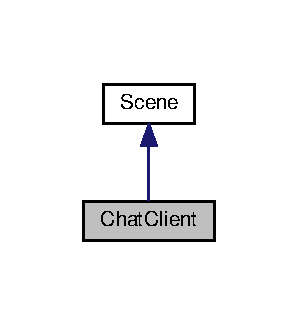
\includegraphics[width=143pt]{classChatClient__inherit__graph}
\end{center}
\end{figure}


Collaboration diagram for Chat\+Client\+:\nopagebreak
\begin{figure}[H]
\begin{center}
\leavevmode
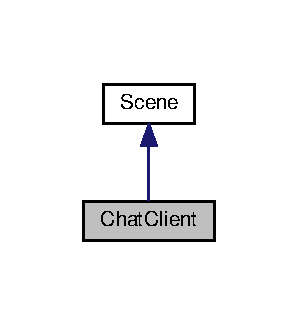
\includegraphics[width=143pt]{classChatClient__coll__graph}
\end{center}
\end{figure}
\subsection*{Public Member Functions}
\begin{DoxyCompactItemize}
\item 
{\bfseries Chat\+Client} (S\+D\+L\+\_\+\+Window $\ast$window, S\+D\+L\+\_\+\+Renderer $\ast$renderer, const std\+::string \&ip\+Address, std\+::uint16\+\_\+t port, const std\+::string \&user\+Name)\hypertarget{classChatClient_ad67333067769e75bbfdbf01c72a0d6c8}{}\label{classChatClient_ad67333067769e75bbfdbf01c72a0d6c8}

\item 
virtual Scene\+Result {\bfseries run} () override\hypertarget{classChatClient_acea2119ab2d1547fa64f481652585533}{}\label{classChatClient_acea2119ab2d1547fa64f481652585533}

\end{DoxyCompactItemize}
\subsection*{Additional Inherited Members}


The documentation for this class was generated from the following files\+:\begin{DoxyCompactItemize}
\item 
chat\+\_\+client.\+h\item 
chat\+\_\+client.\+cpp\end{DoxyCompactItemize}

\hypertarget{classChatMenu}{}\section{Chat\+Menu Class Reference}
\label{classChatMenu}\index{Chat\+Menu@{Chat\+Menu}}


Inheritance diagram for Chat\+Menu\+:\nopagebreak
\begin{figure}[H]
\begin{center}
\leavevmode
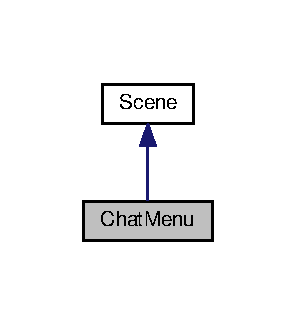
\includegraphics[width=142pt]{classChatMenu__inherit__graph}
\end{center}
\end{figure}


Collaboration diagram for Chat\+Menu\+:\nopagebreak
\begin{figure}[H]
\begin{center}
\leavevmode
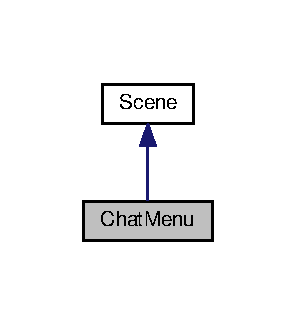
\includegraphics[width=142pt]{classChatMenu__coll__graph}
\end{center}
\end{figure}
\subsection*{Public Member Functions}
\begin{DoxyCompactItemize}
\item 
{\bfseries Chat\+Menu} (S\+D\+L\+\_\+\+Window $\ast$window, S\+D\+L\+\_\+\+Renderer $\ast$renderer)\hypertarget{classChatMenu_a2bc09611256858a93511cbe1601cd201}{}\label{classChatMenu_a2bc09611256858a93511cbe1601cd201}

\item 
virtual Scene\+Result {\bfseries run} () override\hypertarget{classChatMenu_ada4cb8bbf52e735622feeb966c3d38a1}{}\label{classChatMenu_ada4cb8bbf52e735622feeb966c3d38a1}

\end{DoxyCompactItemize}
\subsection*{Additional Inherited Members}


The documentation for this class was generated from the following files\+:\begin{DoxyCompactItemize}
\item 
chat\+\_\+menu.\+h\item 
chat\+\_\+menu.\+cpp\end{DoxyCompactItemize}

\hypertarget{classChatRoomLister}{}\section{Chat\+Room\+Lister Class Reference}
\label{classChatRoomLister}\index{Chat\+Room\+Lister@{Chat\+Room\+Lister}}


Inheritance diagram for Chat\+Room\+Lister\+:\nopagebreak
\begin{figure}[H]
\begin{center}
\leavevmode
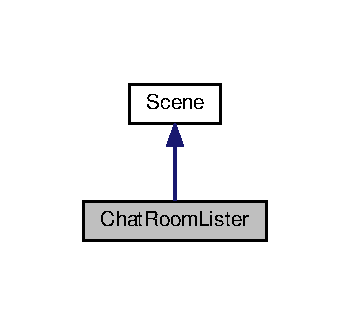
\includegraphics[width=168pt]{classChatRoomLister__inherit__graph}
\end{center}
\end{figure}


Collaboration diagram for Chat\+Room\+Lister\+:\nopagebreak
\begin{figure}[H]
\begin{center}
\leavevmode
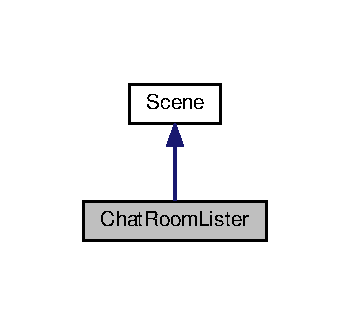
\includegraphics[width=168pt]{classChatRoomLister__coll__graph}
\end{center}
\end{figure}
\subsection*{Public Member Functions}
\begin{DoxyCompactItemize}
\item 
{\bfseries Chat\+Room\+Lister} (S\+D\+L\+\_\+\+Window $\ast$window, S\+D\+L\+\_\+\+Renderer $\ast$renderer)\hypertarget{classChatRoomLister_a1361cdff946e7944ca05bcf05a5cb5c1}{}\label{classChatRoomLister_a1361cdff946e7944ca05bcf05a5cb5c1}

\item 
virtual Scene\+Result {\bfseries run} () override\hypertarget{classChatRoomLister_a9ffee813f6d8c1b9b664771e02f59148}{}\label{classChatRoomLister_a9ffee813f6d8c1b9b664771e02f59148}

\end{DoxyCompactItemize}
\subsection*{Additional Inherited Members}


The documentation for this class was generated from the following files\+:\begin{DoxyCompactItemize}
\item 
chat\+\_\+room\+\_\+lister.\+h\item 
chat\+\_\+room\+\_\+lister.\+cpp\end{DoxyCompactItemize}

\hypertarget{classChatServer}{}\section{Chat\+Server Class Reference}
\label{classChatServer}\index{Chat\+Server@{Chat\+Server}}


Inheritance diagram for Chat\+Server\+:\nopagebreak
\begin{figure}[H]
\begin{center}
\leavevmode
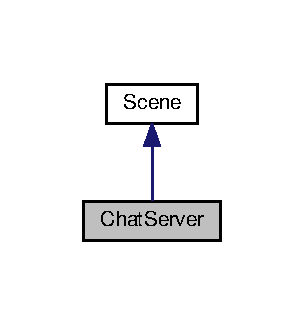
\includegraphics[width=146pt]{classChatServer__inherit__graph}
\end{center}
\end{figure}


Collaboration diagram for Chat\+Server\+:\nopagebreak
\begin{figure}[H]
\begin{center}
\leavevmode
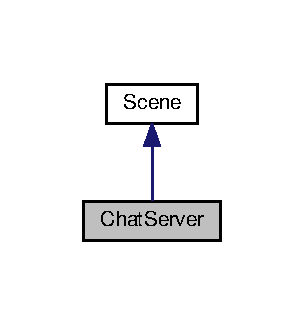
\includegraphics[width=146pt]{classChatServer__coll__graph}
\end{center}
\end{figure}
\subsection*{Public Member Functions}
\begin{DoxyCompactItemize}
\item 
{\bfseries Chat\+Server} (S\+D\+L\+\_\+\+Window $\ast$window, S\+D\+L\+\_\+\+Renderer $\ast$renderer, const std\+::string \&name, std\+::uint16\+\_\+t port, std\+::size\+\_\+t max\+Clients)\hypertarget{classChatServer_a8db1cc9defb74c00f91e68a728ac69e0}{}\label{classChatServer_a8db1cc9defb74c00f91e68a728ac69e0}

\item 
virtual Scene\+Result {\bfseries run} () override\hypertarget{classChatServer_a5da89ab8a56264553c21a4de2124d50a}{}\label{classChatServer_a5da89ab8a56264553c21a4de2124d50a}

\end{DoxyCompactItemize}
\subsection*{Additional Inherited Members}


The documentation for this class was generated from the following files\+:\begin{DoxyCompactItemize}
\item 
chat\+\_\+server.\+h\item 
chat\+\_\+server.\+cpp\end{DoxyCompactItemize}

\hypertarget{classChatServerConfigurator}{}\section{Chat\+Server\+Configurator Class Reference}
\label{classChatServerConfigurator}\index{Chat\+Server\+Configurator@{Chat\+Server\+Configurator}}


Inheritance diagram for Chat\+Server\+Configurator\+:\nopagebreak
\begin{figure}[H]
\begin{center}
\leavevmode
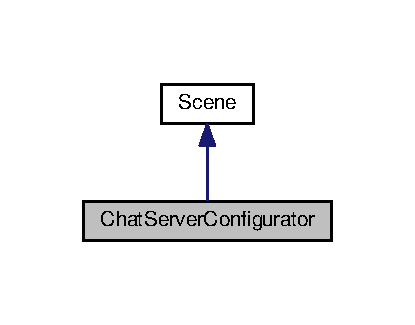
\includegraphics[width=199pt]{classChatServerConfigurator__inherit__graph}
\end{center}
\end{figure}


Collaboration diagram for Chat\+Server\+Configurator\+:\nopagebreak
\begin{figure}[H]
\begin{center}
\leavevmode
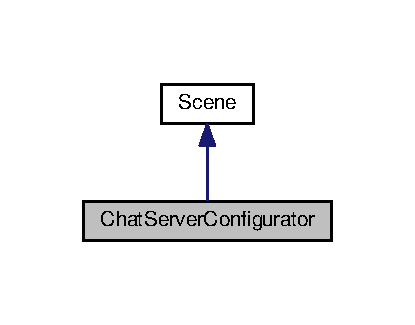
\includegraphics[width=199pt]{classChatServerConfigurator__coll__graph}
\end{center}
\end{figure}
\subsection*{Public Member Functions}
\begin{DoxyCompactItemize}
\item 
{\bfseries Chat\+Server\+Configurator} (S\+D\+L\+\_\+\+Window $\ast$window, S\+D\+L\+\_\+\+Renderer $\ast$renderer)\hypertarget{classChatServerConfigurator_ae05ba01a4fd49b308f38f251a7e2e7d2}{}\label{classChatServerConfigurator_ae05ba01a4fd49b308f38f251a7e2e7d2}

\item 
virtual Scene\+Result {\bfseries run} () override\hypertarget{classChatServerConfigurator_aafcf0a3b741afcde01c174aec1d3112a}{}\label{classChatServerConfigurator_aafcf0a3b741afcde01c174aec1d3112a}

\end{DoxyCompactItemize}
\subsection*{Additional Inherited Members}


The documentation for this class was generated from the following files\+:\begin{DoxyCompactItemize}
\item 
chat\+\_\+server\+\_\+configurator.\+h\item 
chat\+\_\+server\+\_\+configurator.\+cpp\end{DoxyCompactItemize}

\hypertarget{structCurlDeleter}{}\section{Curl\+Deleter Struct Reference}
\label{structCurlDeleter}\index{Curl\+Deleter@{Curl\+Deleter}}
\subsection*{Public Member Functions}
\begin{DoxyCompactItemize}
\item 
void {\bfseries operator()} (C\+U\+RL $\ast$curl)\hypertarget{structCurlDeleter_a772352646fa57a03c2275397326e82b8}{}\label{structCurlDeleter_a772352646fa57a03c2275397326e82b8}

\end{DoxyCompactItemize}


The documentation for this struct was generated from the following file\+:\begin{DoxyCompactItemize}
\item 
kjapp.\+cpp\end{DoxyCompactItemize}

\hypertarget{classScene}{}\section{Scene Class Reference}
\label{classScene}\index{Scene@{Scene}}


Inheritance diagram for Scene\+:\nopagebreak
\begin{figure}[H]
\begin{center}
\leavevmode
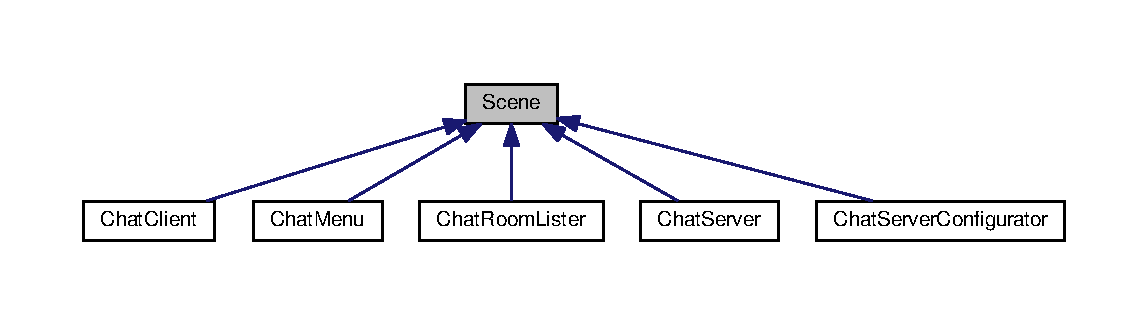
\includegraphics[width=350pt]{classScene__inherit__graph}
\end{center}
\end{figure}
\subsection*{Public Member Functions}
\begin{DoxyCompactItemize}
\item 
{\bfseries Scene} (S\+D\+L\+\_\+\+Window $\ast$window, S\+D\+L\+\_\+\+Renderer $\ast$renderer)\hypertarget{classScene_a833a46b2dfbb25aeb88c281a6926bc17}{}\label{classScene_a833a46b2dfbb25aeb88c281a6926bc17}

\item 
virtual Scene\+Result {\bfseries run} ()=0\hypertarget{classScene_a3ffc2c3184e1fea5a53df4f8190b426b}{}\label{classScene_a3ffc2c3184e1fea5a53df4f8190b426b}

\end{DoxyCompactItemize}
\subsection*{Protected Member Functions}
\begin{DoxyCompactItemize}
\item 
void {\bfseries display\+Text} (const std\+::string \&str, int x\+Pos, int y\+Pos)\hypertarget{classScene_a19f1ae5bf5e6028b07044d5611ffc609}{}\label{classScene_a19f1ae5bf5e6028b07044d5611ffc609}

\item 
void {\bfseries display\+Scroller} ()\hypertarget{classScene_ab819ce5ff68c07408e5c7e8353950220}{}\label{classScene_ab819ce5ff68c07408e5c7e8353950220}

\item 
void {\bfseries draw\+Button} (const S\+D\+L\+\_\+\+Rect \&button, const S\+D\+L\+\_\+\+Color \&color)\hypertarget{classScene_a272378aa86e91b2f24ea8b82989d7bf9}{}\label{classScene_a272378aa86e91b2f24ea8b82989d7bf9}

\item 
void {\bfseries add\+Text\+To\+Scroller} (const std\+::string \&str)\hypertarget{classScene_a5c015411283ae64c0639103ef83eddd6}{}\label{classScene_a5c015411283ae64c0639103ef83eddd6}

\item 
void {\bfseries handle\+Event} (const S\+D\+L\+\_\+\+Event \&event)\hypertarget{classScene_a89937129ba4b9e6d248ec1cb5f2d7147}{}\label{classScene_a89937129ba4b9e6d248ec1cb5f2d7147}

\item 
bool {\bfseries is\+Clicked} (const S\+D\+L\+\_\+\+Rect \&button, const int x\+Pos, const int y\+Pos)\hypertarget{classScene_a29a09821280c1307f198d98edd193870}{}\label{classScene_a29a09821280c1307f198d98edd193870}

\end{DoxyCompactItemize}
\subsection*{Protected Attributes}
\begin{DoxyCompactItemize}
\item 
S\+D\+L\+\_\+\+Window $\ast$ {\bfseries m\+\_\+window}\hypertarget{classScene_a2354b78f3c352a5ee1fb6799464c3679}{}\label{classScene_a2354b78f3c352a5ee1fb6799464c3679}

\item 
S\+D\+L\+\_\+\+Renderer $\ast$ {\bfseries m\+\_\+renderer}\hypertarget{classScene_acd9747c72c40ab7301023a2d132cfa3d}{}\label{classScene_acd9747c72c40ab7301023a2d132cfa3d}

\item 
T\+T\+F\+\_\+\+Font $\ast$ {\bfseries m\+\_\+font} \{\}\hypertarget{classScene_a6070fcce3443855955f61f8c6d796033}{}\label{classScene_a6070fcce3443855955f61f8c6d796033}

\item 
std\+::vector$<$ std\+::string $>$ {\bfseries m\+\_\+scroller\+Strings} \{\}\hypertarget{classScene_aeff40e67af5e2ce0cfaed98d48c446e4}{}\label{classScene_aeff40e67af5e2ce0cfaed98d48c446e4}

\item 
bool {\bfseries m\+\_\+running} \{true\}\hypertarget{classScene_a59073327932c7ac2a6e005a8e41ed9ad}{}\label{classScene_a59073327932c7ac2a6e005a8e41ed9ad}

\item 
bool {\bfseries m\+\_\+continue\+Program} \{true\}\hypertarget{classScene_a03a880626c3317ce115bee5c2a996d45}{}\label{classScene_a03a880626c3317ce115bee5c2a996d45}

\end{DoxyCompactItemize}
\subsection*{Static Protected Attributes}
\begin{DoxyCompactItemize}
\item 
static constexpr int {\bfseries F\+O\+N\+T\+\_\+\+H\+E\+I\+G\+HT} = 18\hypertarget{classScene_a5e583ee7e29312bb52ffd9f5c382887a}{}\label{classScene_a5e583ee7e29312bb52ffd9f5c382887a}

\item 
static constexpr std\+::size\+\_\+t {\bfseries D\+I\+S\+P\+L\+A\+Y\+\_\+\+L\+I\+M\+IT} = 10\hypertarget{classScene_a9f3d25cb3ee314b720a03143df52b4c6}{}\label{classScene_a9f3d25cb3ee314b720a03143df52b4c6}

\item 
static constexpr auto {\bfseries G\+A\+M\+E\+\_\+\+T\+O\+K\+EN} = \char`\"{}59ec8be7890cd692461bb7d4\char`\"{}\hypertarget{classScene_ae5f60b96554e06b172570a2f809bc746}{}\label{classScene_ae5f60b96554e06b172570a2f809bc746}

\end{DoxyCompactItemize}


The documentation for this class was generated from the following files\+:\begin{DoxyCompactItemize}
\item 
scene.\+h\item 
scene.\+cpp\end{DoxyCompactItemize}

%--- End generated contents ---

% Index
\backmatter
\newpage
\phantomsection
\clearemptydoublepage
\addcontentsline{toc}{chapter}{Index}
\printindex

\end{document}
